\documentclass[12pt]{article}
\usepackage{times}
\usepackage[english]{babel}
\usepackage[utf8x]{inputenc}
\usepackage[colorinlistoftodos]{todonotes}
\usepackage[margin=1in]{geometry}
\usepackage{graphicx}
\usepackage{epstopdf}
\usepackage{cite}
\usepackage{listings}
\usepackage{dtklogos}
\usepackage{wrapfig}
\usepackage{subfigure}
\usepackage{amsmath}
\usepackage{amsthm}
\usepackage{amssymb}
\usepackage{amscd}
\usepackage{caption}
\usepackage{etoolbox}
\usepackage{fancyhdr}
\usepackage{stackengine}
\usepackage[export]{adjustbox}
\patchcmd{\thebibliography}{\section*{\refname}}{}{}{}
\usepackage[document]{ragged2e}    %This causes text to left align
\usepackage[colorlinks=true, linkcolor=black,citecolor=black,urlcolor=blue]{hyperref}
\bibliographystyle{IEEEtran}
\extrafloats{100}
\DeclareGraphicsRule{.tif}{png}{.png}{`convert #1 `dirname #1`/`basename #1 .tif`.png}

\title{MCHE 357: Lab 5 & 6}

\begin{document}
\lefthyphenmin3
\righthyphenmin4
% \pretolerance=2000
% \tolerance=500 
% \emergencystretch=10pt
%\raggedright     %Stops LaTeX from automatically hyphenating the right margin to fit better
%Combine this with \usepackage[document]{ragged2e} to get a text align left similar to natural MS Word


%-------------------------------------------------------------
%Start of Paper
%-------------------------------------------------------------

%%%%%%%%%%%%%%%%%%%%%%%%%%%%%%%%%%%%%%%%%%%%%%%%%%%%%%
%%%%%%%%%%%%%%%%%%%%%%% TITLE PAGE %%%%%%%%%%%%%%%%%%%%%%%%
%%%%%%%%%%%%%%%%%%%%%%%%%%%%%%%%%%%%%%%%%%%%%%%%%%%%%%

\begin{titlepage}

\newcommand{\HRule}{\rule{\linewidth}{0.5mm}} % Defines a new command for the horizontal lines, change thickness here

\center % Center everything on the page
 
%----------------------------------------------------------------------------------------
%	Heading Section
%----------------------------------------------------------------------------------------

\textsc{\LARGE University of Louisiana at Lafayette}\\[1.5cm] % Name of your university/college
\textsc{\Large Measurements and Instrumentation}\\[0.5cm] % Major heading such as course name
\textsc{\large MCHE 357}\\[0.5cm] % Minor heading such as course title

%----------------------------------------------------------------------------------------
%	Title Section
%----------------------------------------------------------------------------------------

\HRule \\[0.4cm]
{ \huge \bfseries Lab 5 \& 6}\\[0.4cm] % Title of your document
\HRule \\[1.5cm]
 
%----------------------------------------------------------------------------------------
%	Author Section
%----------------------------------------------------------------------------------------

\begin{minipage}{0.4\textwidth}
\begin{flushleft} \large
\emph{Author:}\\
\textsc{Matthew J. Begneaud} \\% Your name
\end{flushleft}
\end{minipage}
~
\begin{minipage}{0.4\textwidth}
\begin{flushright} \large
\emph{Professor:} \\
\textsc{Dr. Mostafa A. Elsayed} % Supervisor's Name
\end{flushright}
\end{minipage}\\[1.5cm]

% If you don't want a supervisor, uncomment the two lines below and remove the section above
%\Large \emph{Author:}\\
%John \textsc{Smith}\\[3cm] % Your name

%----------------------------------------------------------------------------------------
%	Date Section
%----------------------------------------------------------------------------------------

{\textsc{\large \today}}\\[0.5cm] % Date, change the \today to a set date if you want to be precise


%----------------------------------------------------------------------------------------
%	Group Section
%----------------------------------------------------------------------------------------
% No group for this lab
%\textsc{\large Group:}\\[0.1cm]
%\textsc{Ronald Kisor}\\
%\textsc{Chandler Lagarde}\\
%\textsc{Somto Umeokafor}
%\\[0.5cm]

%----------------------------------------------------------------------------------------
%	Logo Section
%----------------------------------------------------------------------------------------


\includegraphics[width=5in]{UL_logo.jpg}\\[1cm] % Include a department/university logo - this will require the graphicx package
 
%----------------------------------------------------------------------------------------

\vfill % Fill the rest of the page with whitespace

\end{titlepage}

%%%%%%%%%%%%%%%%%%%%%%%%%%%%%%%%%%%%%%%%%%%%%%%%%%%%%%
%%%%%%%%%%%%%%%%%%%%%%% TABLE OF CONTENTS %%%%%%%%%%%%%%%%%%%
%%%%%%%%%%%%%%%%%%%%%%%%%%%%%%%%%%%%%%%%%%%%%%%%%%%%%%

\tableofcontents

\listoffigures

\bigskip


\section*{\fontsize{12}{12}\selectfont \large List of Symbols}
\addcontentsline{toc}{section}{List of Symbols} % Add for each section
None




\newpage

%%%%%%%%%%%%%%%%%%%%%%%%%%%%%%%%%%%%%%%%%%%%%%%%%%%%%%
%%%%%%%%%%%%%%%%%%%%%%% REPORT %%%%%%%%%%%%%%%%%%%%%%%%%%
%%%%%%%%%%%%%%%%%%%%%%%%%%%%%%%%%%%%%%%%%%%%%%%%%%%%%%


\section*{\fontsize{12}{12}\selectfont \large Introduction}
\addcontentsline{toc}{section}{Introduction} % Add for each section
This two part lab consisted of using a program created in Lab View in Lab 5. This program was used to take data in from a physical system in the lab and plot the data. The system contains a photo-resistor which changes resistance depending on the amount of light it is exposed to.


\section*{\fontsize{12}{12}\selectfont \large Theory}
\addcontentsline{toc}{section}{Theory} % Add for each section
Lab View is used to simulate real control systems, and consists of many optional devices and operations that can be used in the simulations. In control systems, typically data is read in from sensors and is then sent through different devices and controllers to give a desired output or feedback. Some examples of operations are summing two or more inputs, converting data units, performing FFT analysis, passing signals through filters, and plotting data back to the user if information about a signal is required.
\bigskip

FFT is a computational method which performs a Fourier Transform by using computational tricks to speed up the calculation rather than try to actually solve differential equations. The FFT technique is implemented in order to measure the natural frequency of a system. This is done typically by returning a set of frequencies along with magnitudes that correspond to these frequencies. The frequencies with the highest magnitudes are considered the "dominant" frequencies of a system, and indicate which frequencies the system naturally vibrates with.
\bigskip

A photo-resistor is a device which changes its resistance based on the amount of light it is exposed to. This can be used to measure the frequency with which a light is switching on and off for example. The frequency with which the resistance changes matches the lighting frequency.


\section*{\fontsize{12}{12}\selectfont \large Procedure \& Analysis}
\addcontentsline{toc}{section}{Procedure \& Analysis} % Add for each section

The program created in Lab View can be seen in Figure 1 and Figure 2. In the physical part of the lab, the photo-resistor was initially wired up as part of a Wheatstone Bridge and was tested. A droplight was shone on the device and the resistance was measured, shown in Figure 3. The light was then turned off to see the significant change in resistance.
\bigskip

In the program, physical channel inputs were initiated and are set up to take in data from a physical system. A flashlight was then shone on the photo-resistor through a circular fan, which caused the light to blink on the photo-resistor. This can be seen in Figure 4. The frequency of blinking depends on the speed of the fan and the number of blades on the fan. The Lab View program was used to record and save the data from this experiment, and is plotted in Figure 5. 
\bigskip

A strobe light with a user-selectable blink frequency, called a stroboscope, was then shone on the photo-resistor, shown in Figure 6. This data was also recorded and saved, and is plotted in Figure 7. The same stroboscope was then shown on the oscillating fan, which has a hole in on of its blades. The frequency of the flashlight was then matched to the frequency of the holed-blade making one complete revolution. This caused the blade to appear to stay in one spot, as shown in Figure 8.
\bigskip
 
 \newpage
 
 \begin{figure}[h!] %  figure placement: here, top, bottom, or page
   \centering
   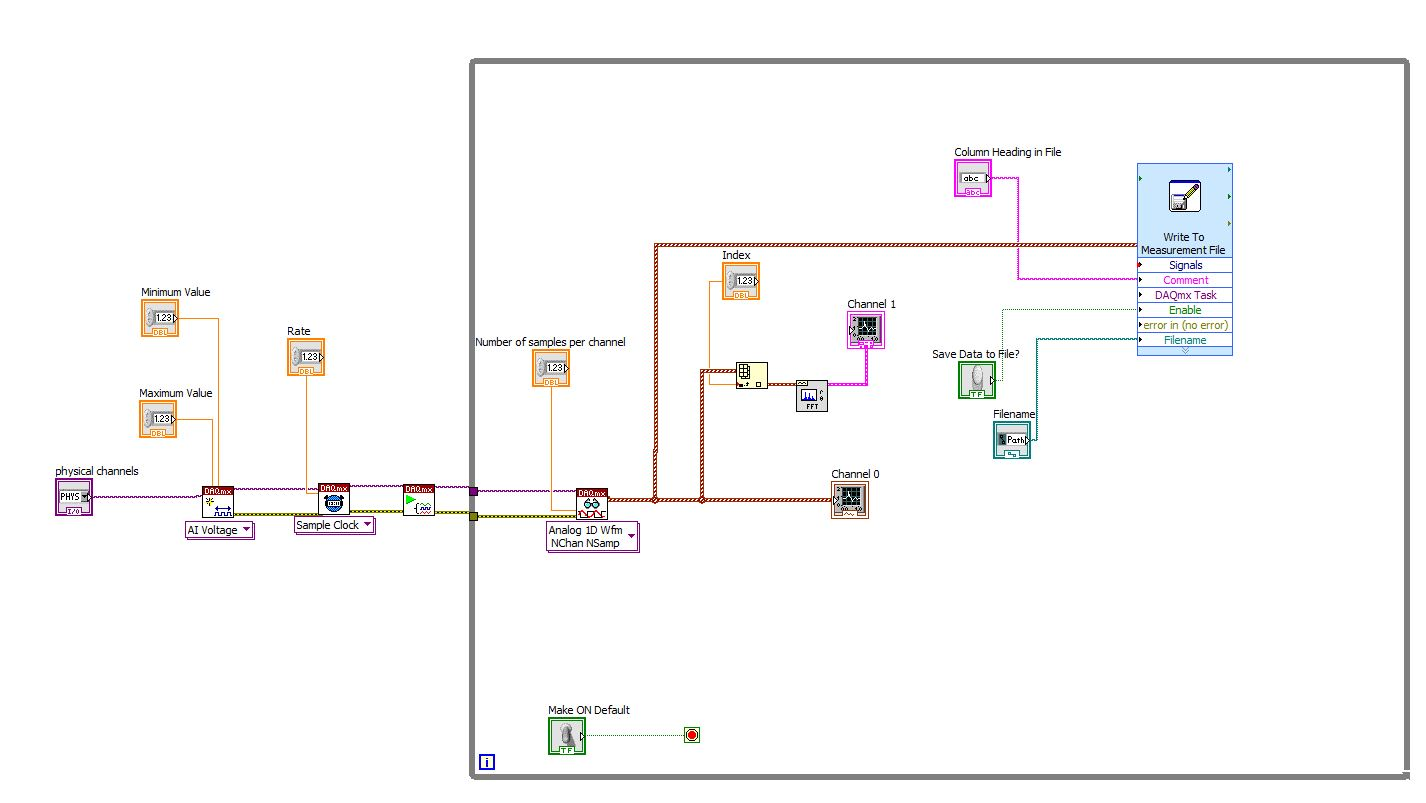
\includegraphics[width=5in]{Lab5BackPanel.JPG} 
   \caption{System Diagram}
   \label{fig:example}
\end{figure}


\begin{figure}[h!] %  figure placement: here, top, bottom, or page
   \centering
   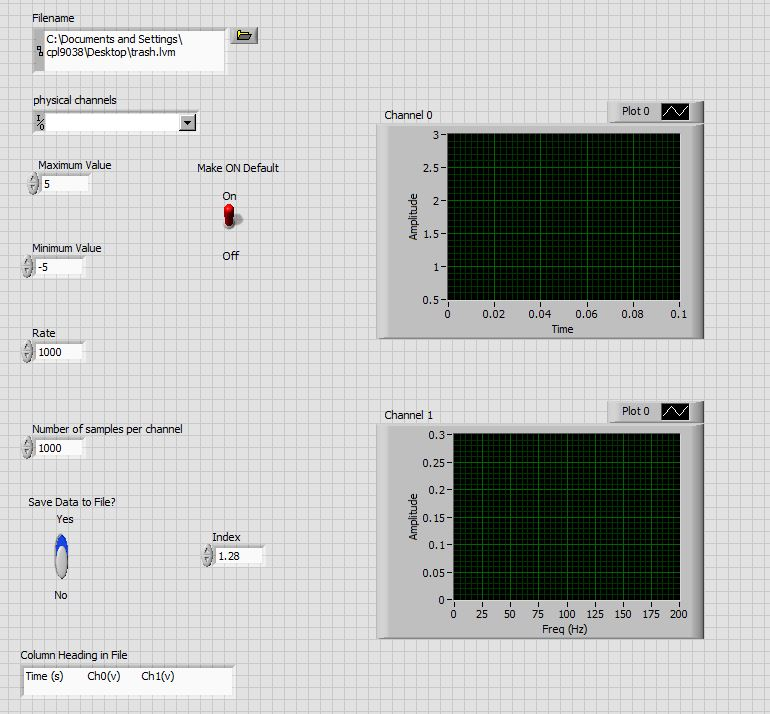
\includegraphics[width=5in]{Lab5FrontPanel.JPG} 
   \caption{Control Panel \& Chart Readout}
   \label{fig:example}
\end{figure}

\newpage
 
\begin{figure}[h!] %  figure placement: here, top, bottom, or page
   \centering
   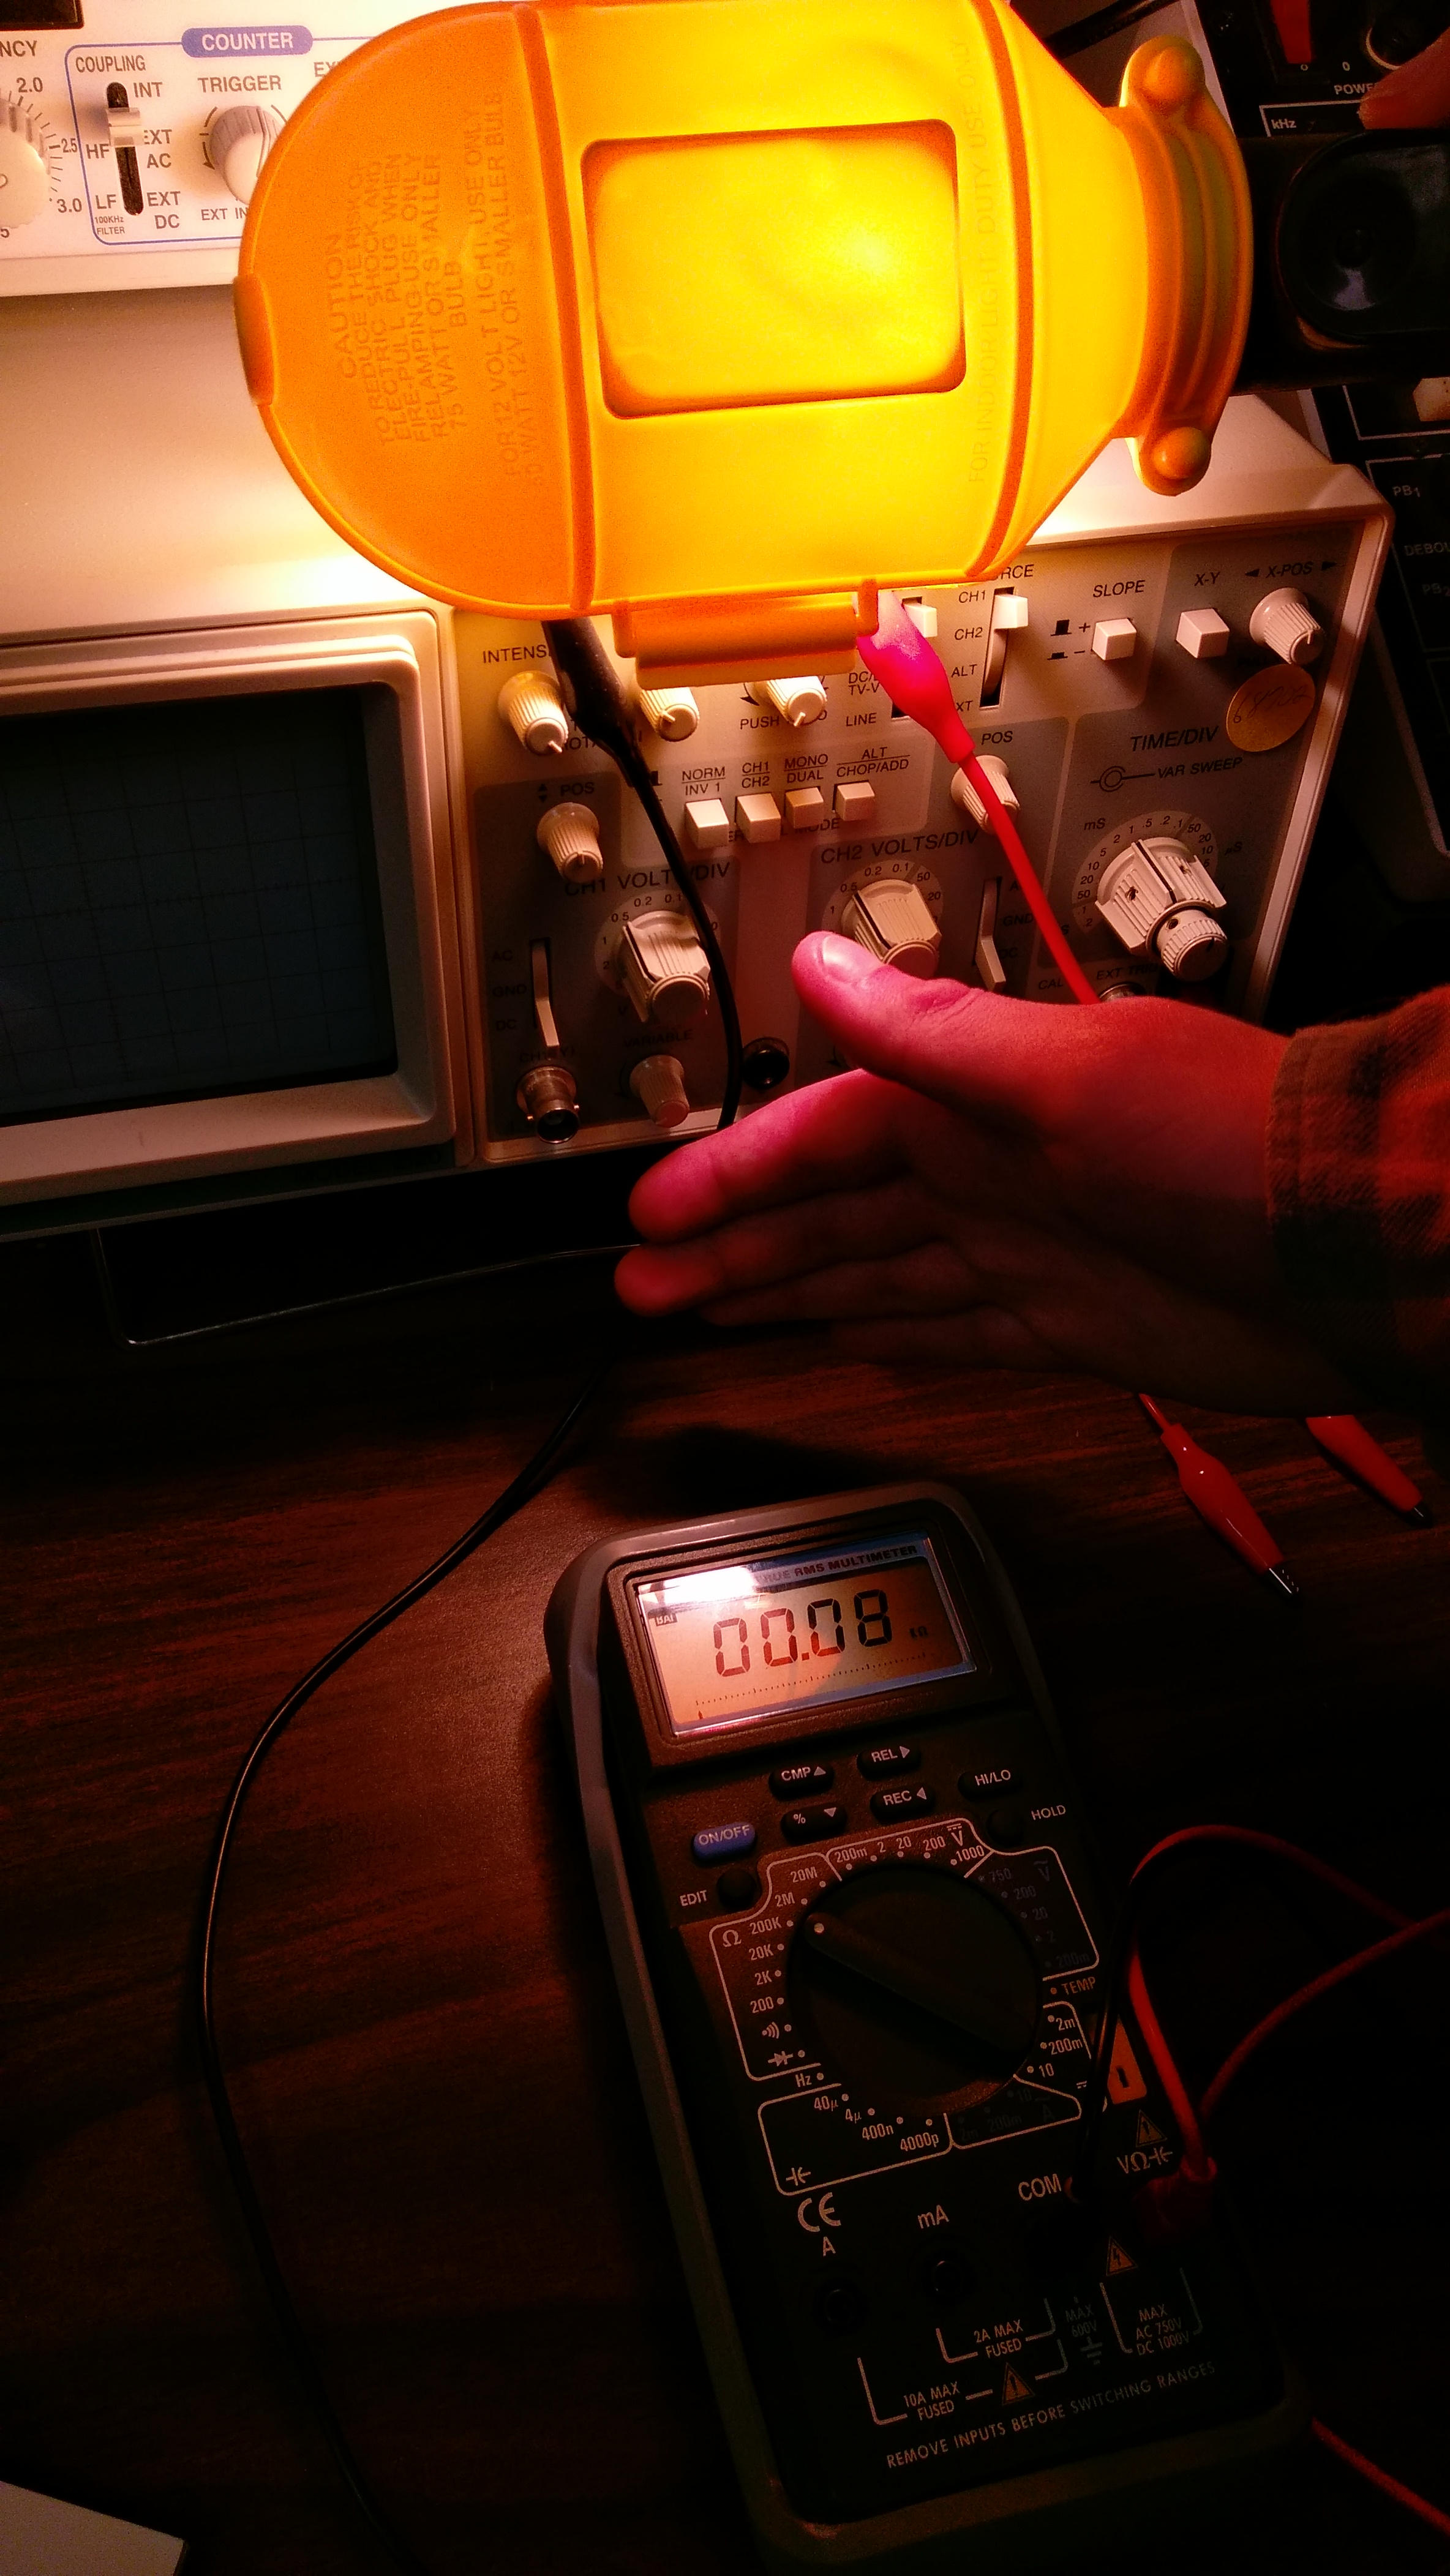
\includegraphics[width=2in]{droplight_resistance.jpg} 
   \caption{Droplight on Photo-Resistor}
   \label{fig:example}
\end{figure}

\bigskip

\begin{figure}[h!] %  figure placement: here, top, bottom, or page
   \centering
   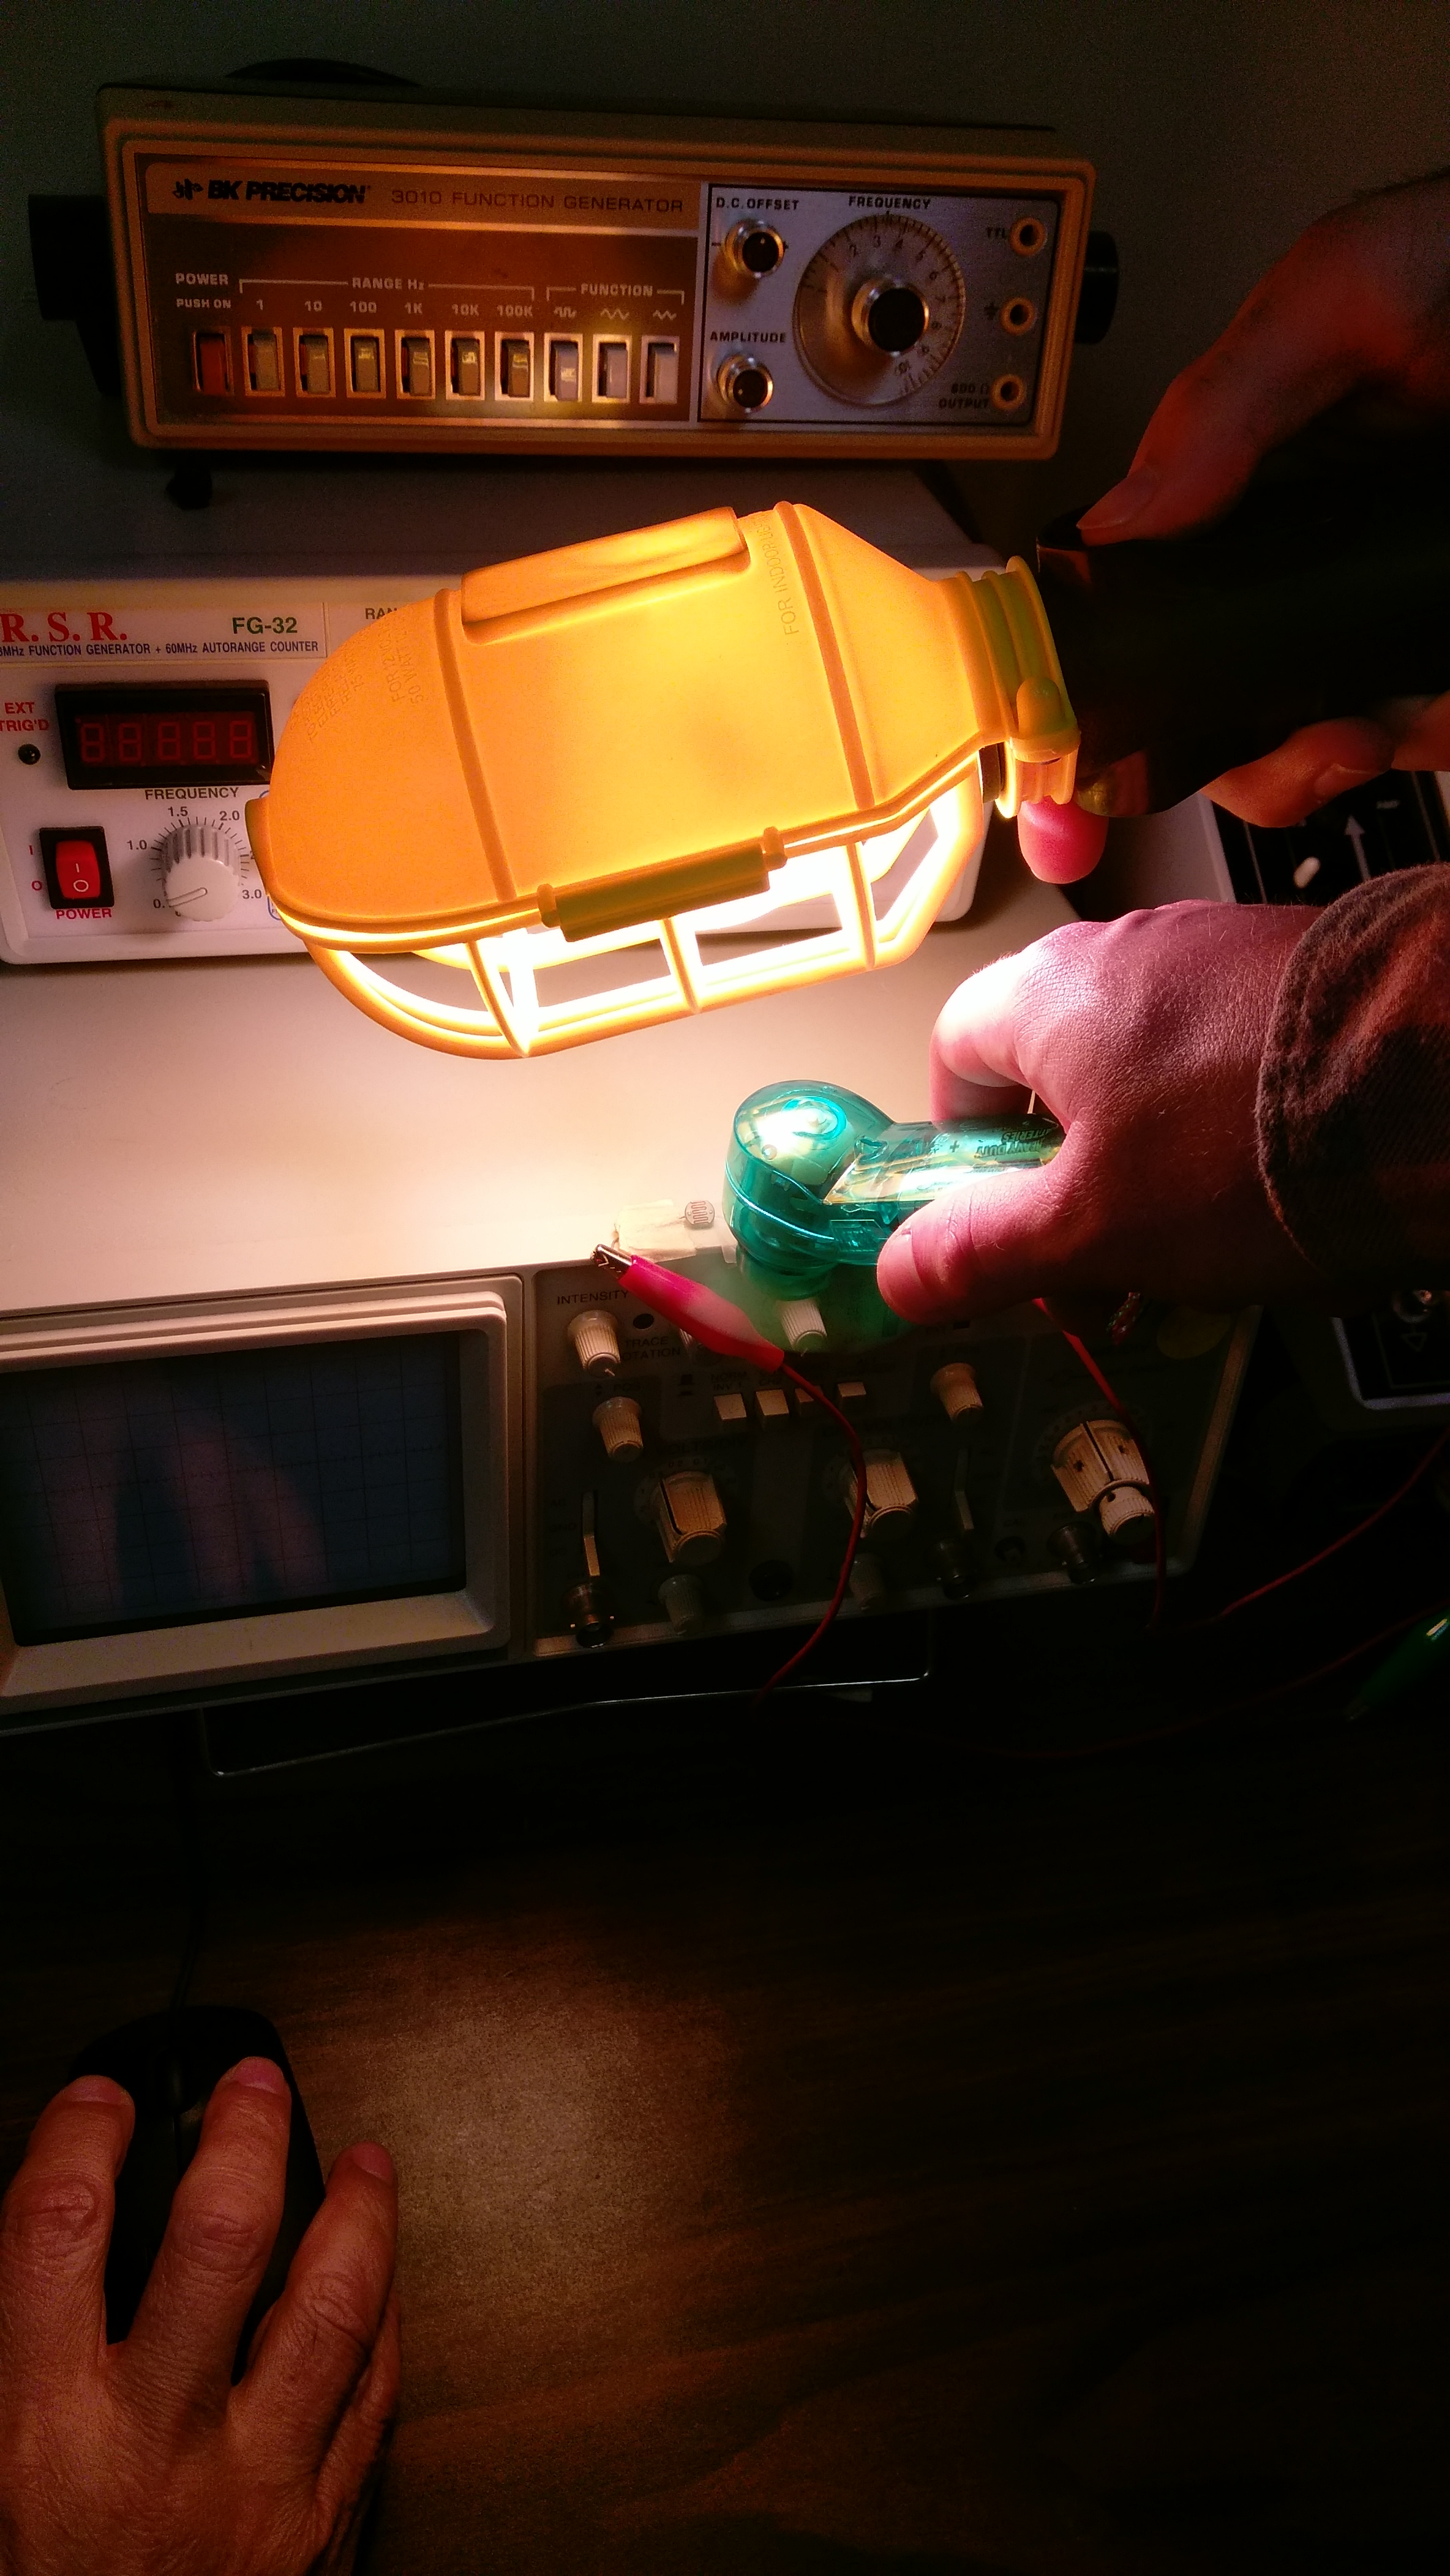
\includegraphics[width=2in]{droplight_fan_photoresistor.jpg} 
   \caption{Droplight on Photo-Resistor through Fan}
   \label{fig:example}
\end{figure}

\newpage

\begin{figure}[h!] %  figure placement: here, top, bottom, or page
   \centering
   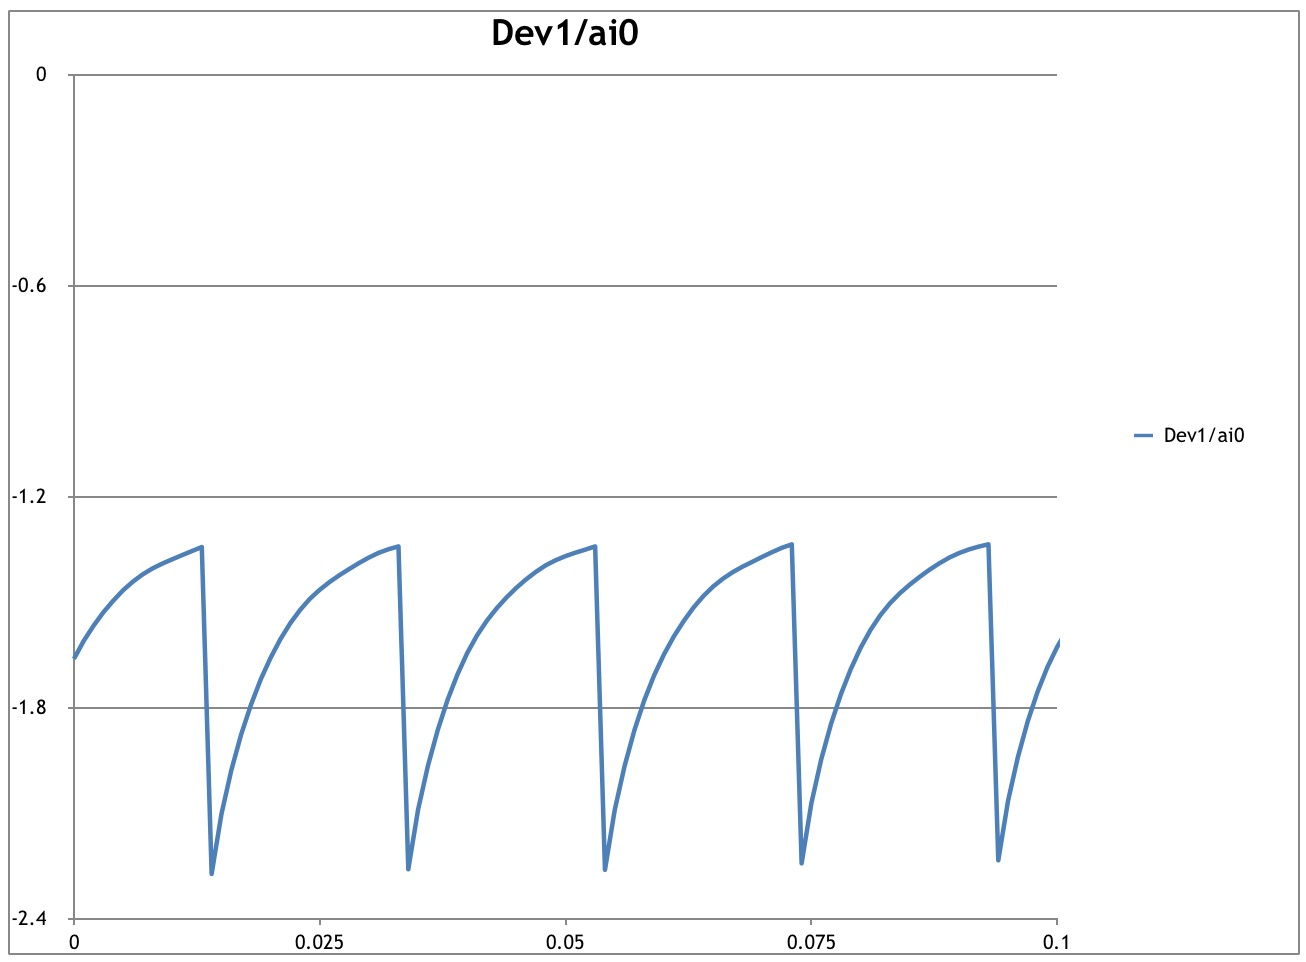
\includegraphics[width=5in]{data1_plot.jpg} 
   \caption{Data Plot for Droplight-Fan Experiment}
   \label{fig:example}
\end{figure}

\bigskip

\begin{figure}[h!] %  figure placement: here, top, bottom, or page
   \centering
   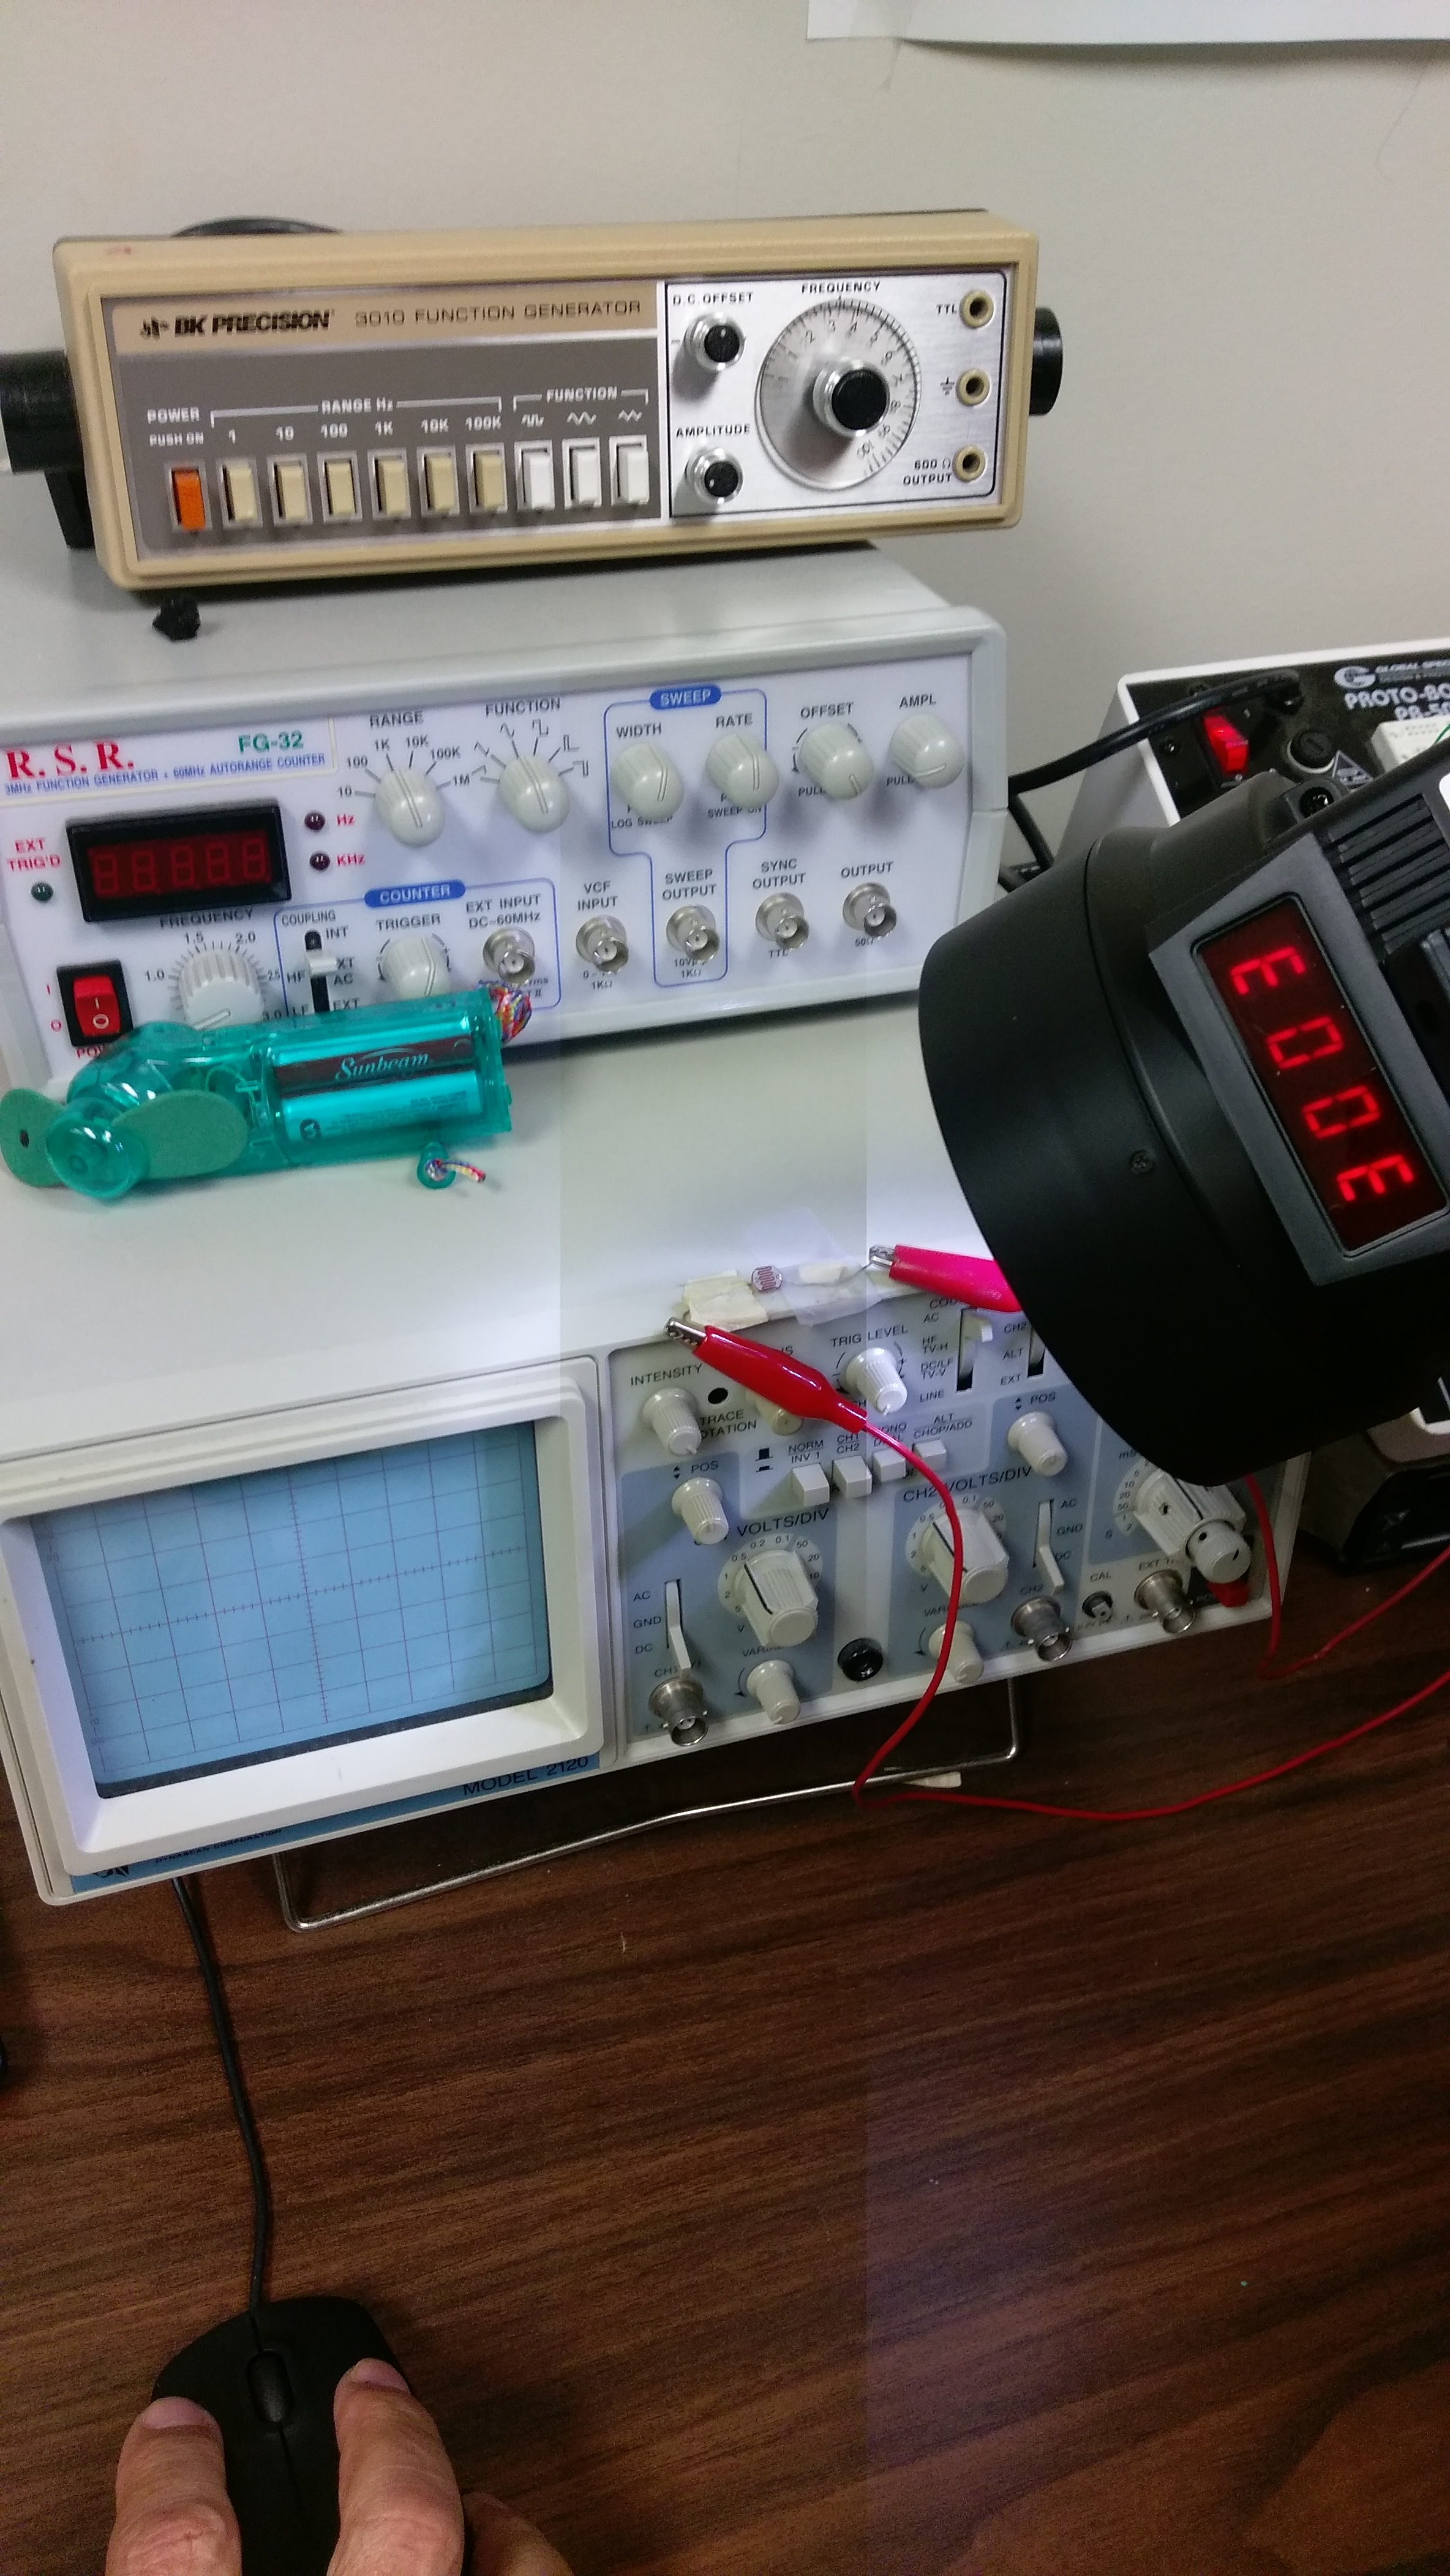
\includegraphics[width=2in]{strobe_light_photoresistor.jpg} 
   \caption{Stroboscope on Photo-Resistor}
   \label{fig:example}
\end{figure}

\newpage

\begin{figure}[h!] %  figure placement: here, top, bottom, or page
   \centering
   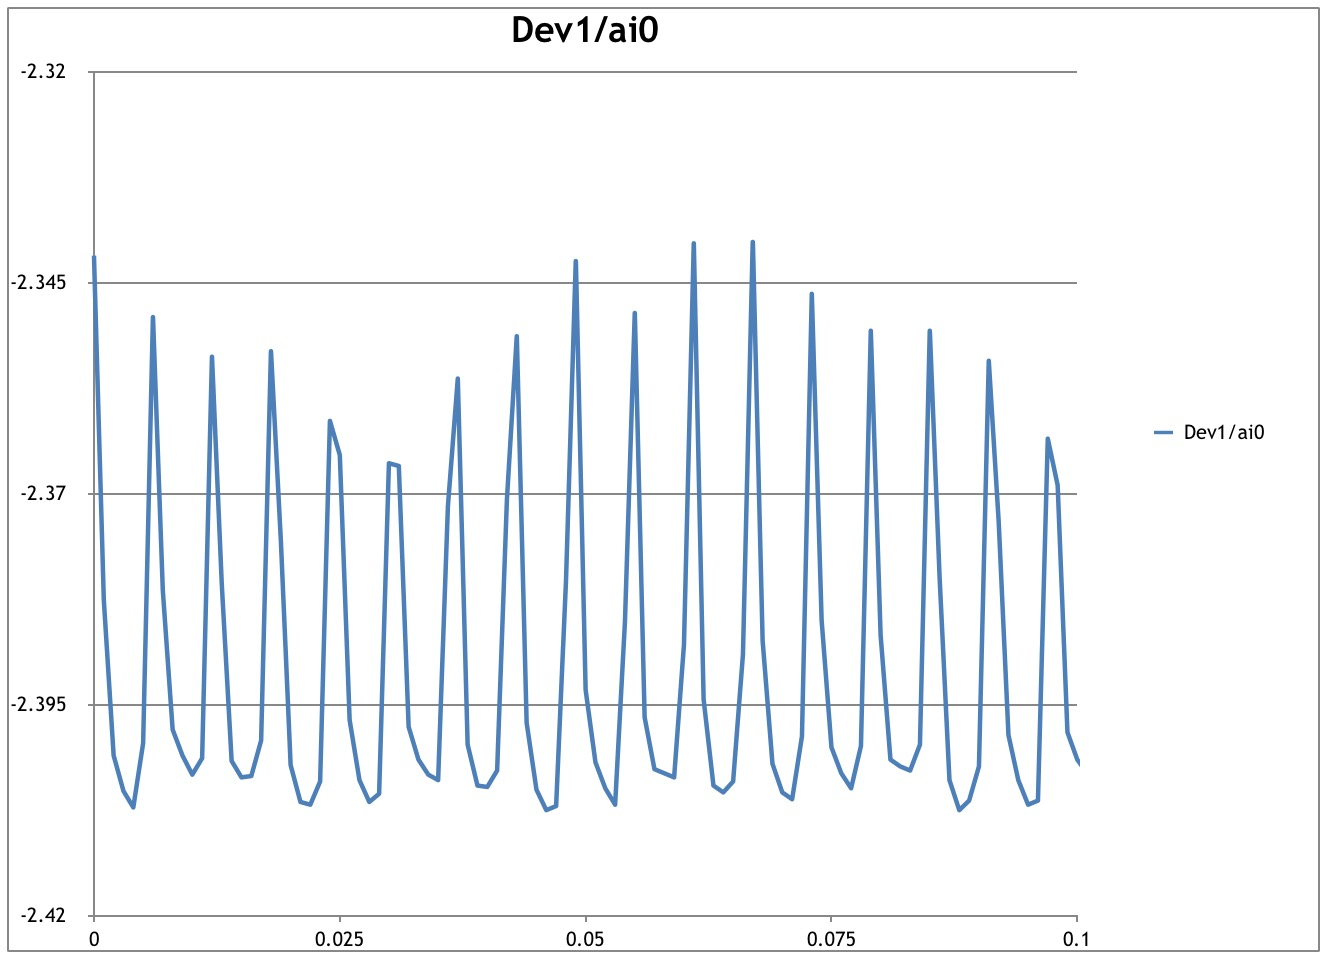
\includegraphics[width=5in]{data2_plot.jpg} 
   \caption{Data Plot for Stroboscope on Photo-Resistor}
   \label{fig:example}
\end{figure}

\bigskip

\begin{figure}[h!] %  figure placement: here, top, bottom, or page
   \centering
   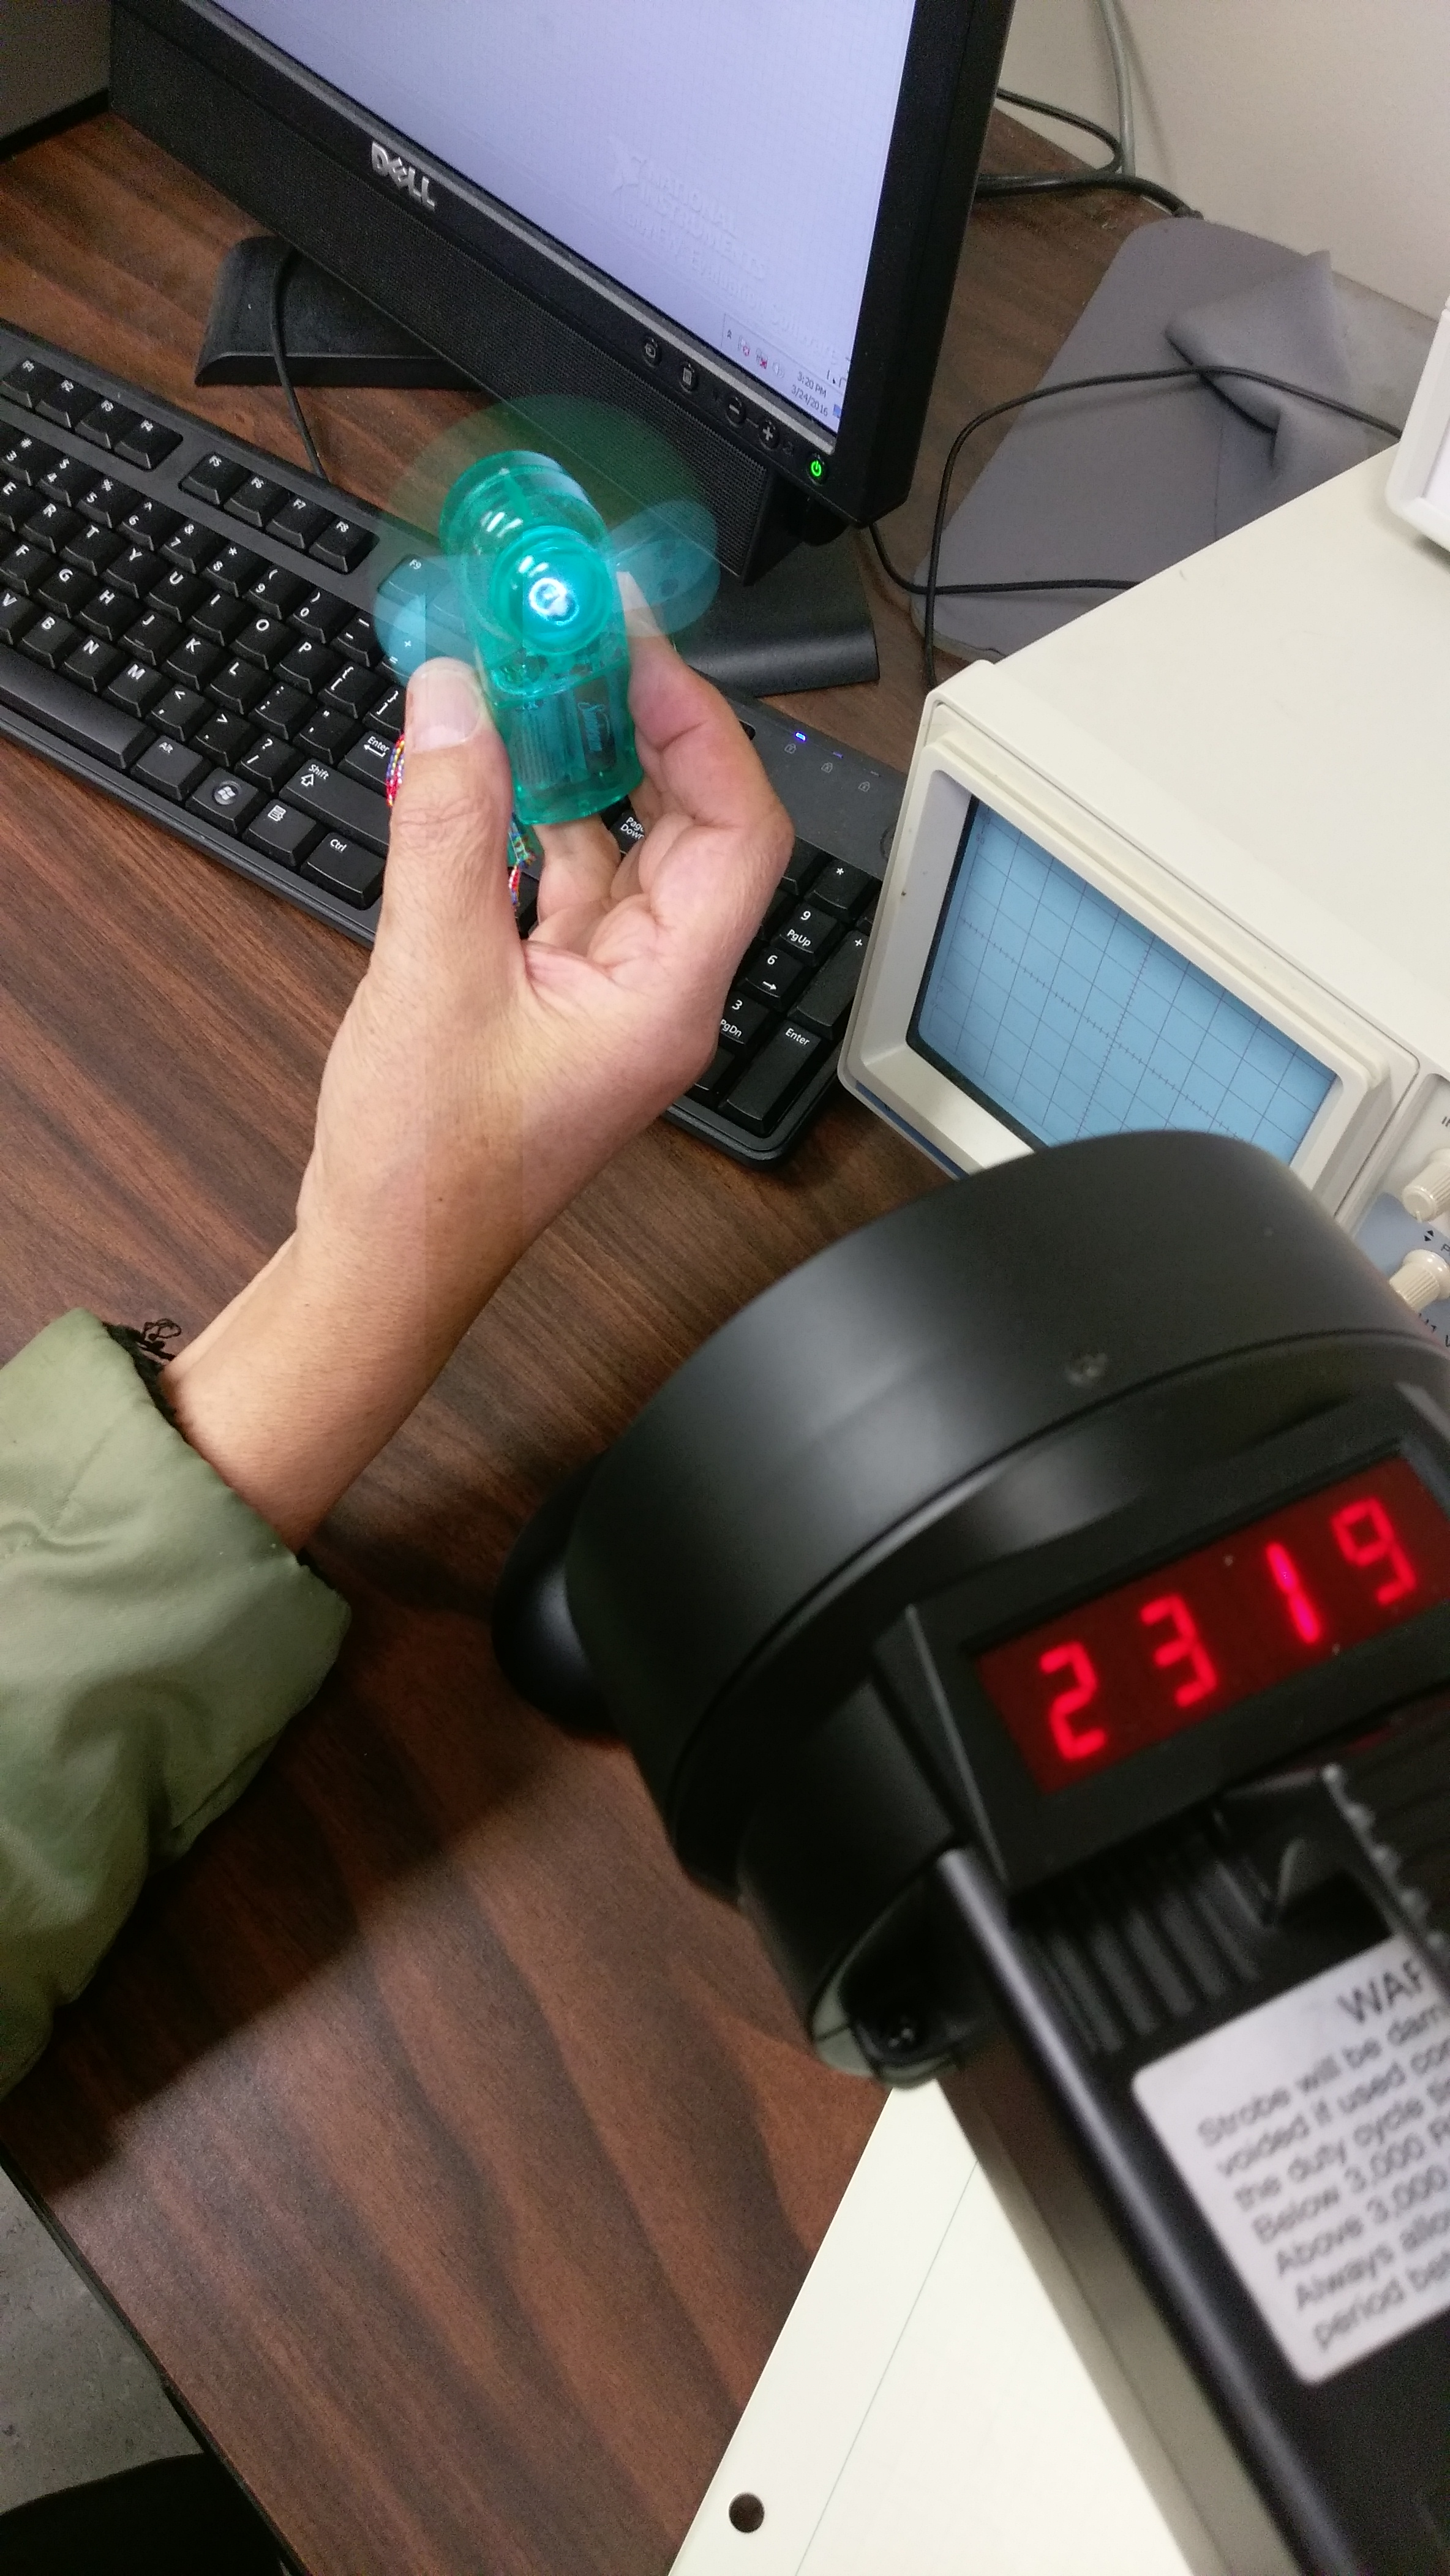
\includegraphics[width=2in]{fan_frequency_match.jpg} 
   \caption{Frequency Match Between Fan and Stroboscope}
   \label{fig:example}
\end{figure}

\newpage

\section*{\fontsize{12}{12}\selectfont \large Conclusion}
\addcontentsline{toc}{section}{Conclusion} % Add for each section
The exercises conducted in this lab demonstrated the task of measuring frequency. In this case, the frequency of a light was measured, but similar skills and program could be applied to a different type of harmonic system by using a different means of sensing oscillations. This lab also demonstrated how to use Lab View programs with a physical system, which is what Lab View is used for widely in industry.



%\section*{\fontsize{12}{12}\selectfont \large References}

%\begin{thebibliography}{2}
%
%% Example
%%\bibitem{Wagner}
%%Ng, K., Wagner, S.W., Camelio, J., Emblom, W.J. (2010). ?Experimental Analysis of Micro Tube
%%Hydroforming Process.? Transactions of NAMRC of SME, 38, 577-584.
%
%\end{thebibliography}



%\section*{\fontsize{12}{12}\selectfont APPENDIX}

%\begin{table}[h!]
%  \caption{}
%  \includegraphics[width=\linewidth]{table1.png}
%\end{table}




\end{document}







----------------------------Templates-------------------------------

-------------------------Figure-----------------------

\begin{figure}[h!]  
  \centering
    \includegraphics[width=\linewidth]{**file**}
    \caption{Docking Station}
\end{figure}

---------------------------Table-----------------------
\begin{table}[ht]
\caption{Nonlinear Model Results} % title of Table
\centering % used for centering table
\begin{tabular}{c c c c} % centered columns (4 columns)
\hline\hline %inserts double horizontal lines
Case & Method\#1 & Method\#2 & Method\#3 \\ [0.5ex] % inserts table
%heading
\hline % inserts single horizontal line
1 & 50 & 837 & 970 \\ % inserting body of the table
2 & 47 & 877 & 230 \\
3 & 31 & 25 & 415 \\
4 & 35 & 144 & 2356 \\
5 & 45 & 300 & 556 \\ [1ex] % [1ex] adds vertical space
\hline %inserts single line
\end{tabular}
\label{table:nonlin} % is used to refer this table in the text
\end{table}



probably best to insert as an image from excel

\bigskip\\
\begin{table}[h!]
  \caption{}
  \includegraphics[width=\linewidth]{**file**}
\end{table}
\bigskip\\





-----------------------------Equations------------------------
-----------------------------Regular
\begin{equation}
a = b + c
\end{equation}

--------------------------------- Multiline
\begin{multline}
a = b + c + d + e + f
+ g + h + i + j \\
+ k + l + m + n + o
\end{multline}

-------------------------------Citations-------------------------
\bibitem{Author last name}
  Last, First., year of publication,
  article name, book(etc) name, from \\
  link goes here

----------------------------------other-----------------------------

equations:
http://moser-isi.ethz.ch/docs/typeset_equations.pdf

citations:
http://library.missouri.edu/engineering/about/guides/asme
https://www.asme.org/shop/proceedings/conference-publications/references